\documentclass[11pt,a4paper]{ivoa}
\input tthdefs

\title{Catalogue of User Defined Functions}

% see ivoatexDoc for what group names to use here
\ivoagroup{DAL}

%\author[????URL????]{????Alfred Usher Thor????}
\author{Markus Demleitner}
\author{Jon Juaristi Campillo}


\editor{Markus Demleitner}

% \previousversion[????URL????]{????Funny Label????}
\previousversion{This is the first public release}
       

\begin{document}
\begin{abstract}
In these document the official IVOA sanctioned User Defined Functions
(UDF) are listed. The functions must be prefixed by ``ivo\_`` as
defined in the standard. Should more be defined for future use, they
will be written down in this note.
\end{abstract}


%i\section*{Acknowledgments}

%???? Or remove the section header ????

\section*{Conformance-related definitions}

The words ``MUST'', ``SHALL'', ``SHOULD'', ``MAY'', ``RECOMMENDED'', and
``OPTIONAL'' (in upper or lower case) used in this document are to be
interpreted as described in IETF standard RFC2119 \citep{std:RFC2119}.

The \emph{Virtual Observatory (VO)} is a
general term for a collection of federated resources that can be used
to conduct astronomical research, education, and outreach.
The \href{http://www.ivoa.net}{International
Virtual Observatory Alliance (IVOA)} is a global
collaboration of separately funded projects to develop standards and
infrastructure that enable VO applications.


\section{Introduction}

After more than a decade since the foundation of the IVOA, multiple
Virtual Observatories across the world have adapted its standards. In
this case, TAP and query language, ADQL. Due to some of the
functionality not being present in the standards, IVOA defined some UDF
which help users obtain HealPix maps for instance. Despite this, and due
to different services working in different context, there is disparity
on UDF.

In this note we intend to compile those which can be service-independent
but adoptable by anyone who deems it necessary.

%\subsection{Role within the VO Architecture}

%\begin{figure}
\centering

%% As of ivoatex 1.2, the architecture diagram is generated by ivoatex in
% SVG; copy ivoatex/archdiag-full.xml to archdiag.xml and throw out
% all lines not relevant to your standard.
% Notes don't generally need this.  If you don't copy archdiag.xml,
% you must remove archdiag.svg from FIGURES in the Makefile.

%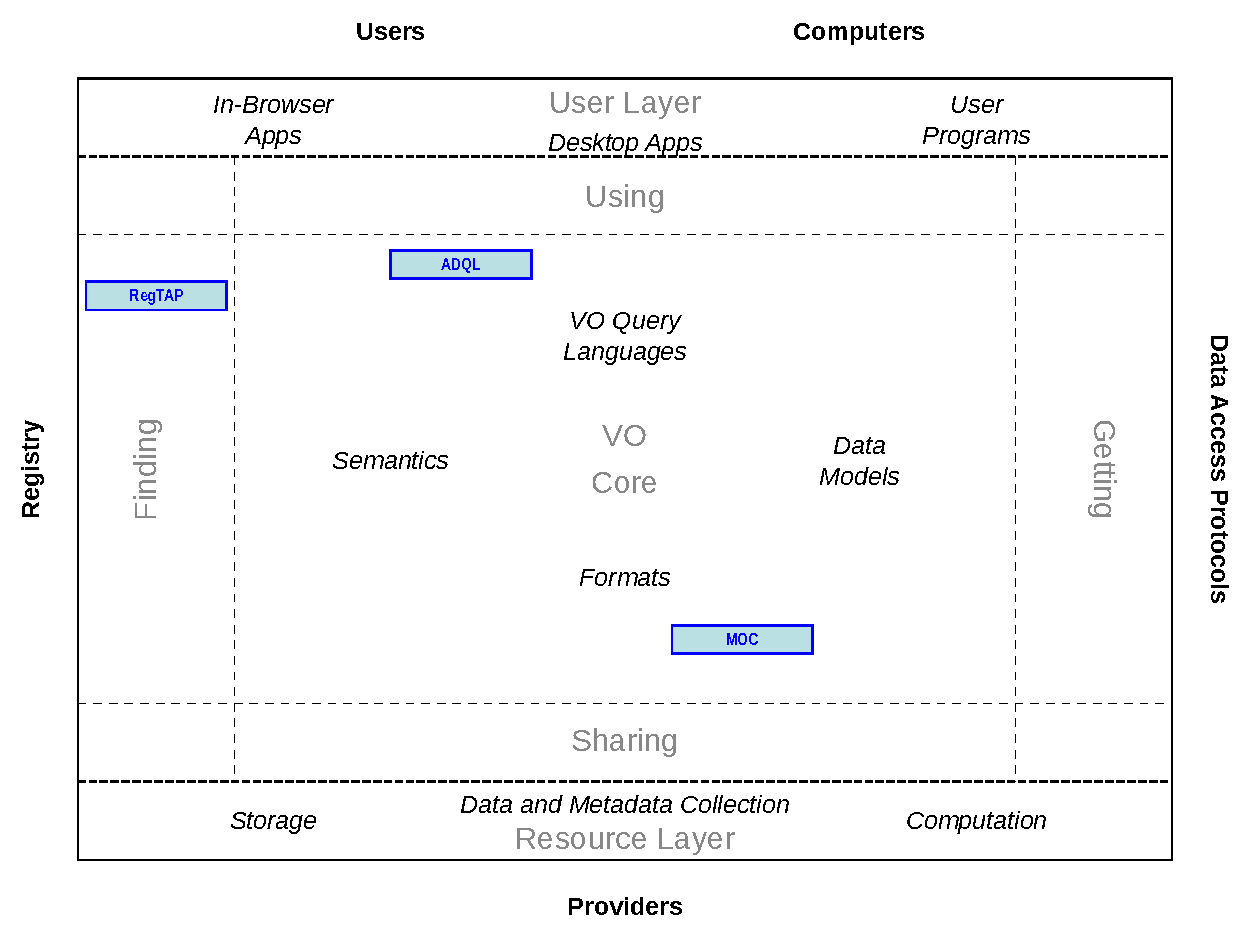
\includegraphics[width=0.9\textwidth]{role_diagram.pdf}
%\caption{Architecture diagram for this document}
%\label{fig:archdiag}
%\end{figure}

%Fig.~\ref{fig:archdiag} shows the role this document plays within the
%IVOA architecture \citep{note:VOARCH}.

%???? and so on, LaTeX as you know and love it. ????

\section{List of user defined functions}
\subsection{Healpix related}
\subsubsection{\texttt{ivo\_healpix\_index} with ra and dec}

Parameters:

\begin{itemize}
	\item hpxOrder (\texttt{INTEGER})
	\item ra (\texttt{DOUBLE})
	\item dec (\texttt{DOUBLE})
\end{itemize}

Returns the index of the (nest) Healpix cell (at the specified order
hpxOrder) containing the specified spherical point defined as a right
ascension and declination value.

\subsubsection{\texttt{ivo\_healpix\_index} with an spherical point}

Parameters:

\begin{itemize}
	\item hpxOrder (\texttt{INTEGER})
	\item point (\texttt{POINT})
\end{itemize}

Returns the index of the (nest) Healpix cell (at the specified order
hpxOrder) containing the specified spherical point.

\subsubsection{ivo\_healpix\_center}

Parameters:

\begin{itemize}
	\item hpxOrder (\texttt{INTEGER})
	\item hpxIndex (\texttt{INTEGER})
\end{itemize}

Returns a \texttt{POINT} corresponding to the center of the Healpix cell
with the given index at the given order.

\subsubsection{\texttt{ivo\_apply\_pm}}

Parameters:

\begin{itemize}
	\item ra (\texttt{DOUBLE})
	\item dec (\texttt{DOUBLE})
	\item pmra (\texttt{DOUBLE})
	\item pmdec (\texttt{DOUBLE})
	\item epochDist (\texttt{DOUBLE})
\end{itemize}

Returns a \texttt{POINT} for a given proper motion (prma and pmdec)
after a given number of Julian years. Positions must be in degrees,
poper motions are expected in degrees/year. Pmra is assumed to contain
cos(delta).

\appendix
\section{Changes from Previous Versions}

No previous versions yet.  
% these would be subsections "Changes from v. WD-..."
% Use itemize environments.


\bibliography{ivoatex/ivoabib,ivoatex/docrepo}


\end{document}
